\documentclass[tikz,convert=false]{standalone}

\usepackage{tikz}
\usepackage{ifthen}
\usetikzlibrary{arrows}

\begin{document}

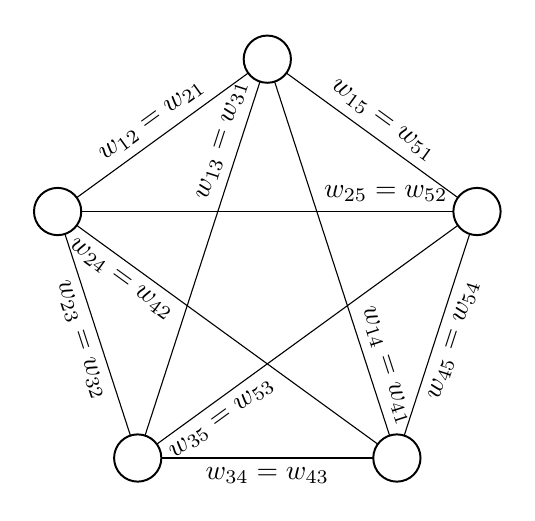
\begin{tikzpicture}
[connection/.style={-,shorten >=0.5pt},
invisible/.style={circle,draw=white,fill=white,inner sep=0pt,minimum size=0mm,line width=0mm},
neuron/.style={circle,draw=black,fill=white,inner sep=0pt,minimum size=6mm,line width=0.25mm}]

\def \numNeurons {5}
\def \radius{2.8}

\def \degreeSeparation {360/\numNeurons}
\pgfmathsetmacro\offset{90-\degreeSeparation}

% Drawing connections
\foreach \neuron in {1,...,\numNeurons} {
	\pgfmathsetmacro\degrees{\degreeSeparation*\neuron+\offset}
	\node[invisible] (\neuron) at (\degrees:\radius) {};
	\node[invisible] at (\degrees:3.2) {};
}

\draw[connection] (1) -- (2) node [midway, sloped,anchor=center, above] {$w_{12}=w_{21}$};
\draw[connection] (1) -- (3) node [at start, above left, sloped, xshift=-0.25cm] {$w_{13}=w_{31}$};
\draw[connection] (1) -- (4) node [at end, above left, sloped, xshift=-0.25cm] {$w_{14}=w_{41}$};
\draw[connection] (1) -- (5) node [midway, sloped,anchor=center, above] {$w_{15}=w_{51}$};
\draw[connection] (2) -- (3) node [midway, sloped,anchor=center, below] {$w_{23}=w_{32}$};
\draw[connection] (2) -- (4) node [at start, below right, sloped,xshift=0.25cm] {$w_{24}=w_{42}$};
\draw[connection] (2) -- (5) node [at end, above left, sloped,xshift=-0.25cm] {$w_{25}=w_{52}$};
\draw[connection] (3) -- (4) node [midway, sloped,anchor=center, below] {$w_{34}=w_{43}$};
\draw[connection] (3) -- (5) node [at start, below right, sloped,xshift=0.25cm] {$w_{35}=w_{53}$};
\draw[connection] (4) -- (5) node [midway, sloped,anchor=center, below] {$w_{45}=w_{54}$};


% Drawing neurons
\foreach \neuron in {1,...,\numNeurons} {
	\pgfmathsetmacro\degrees{\degreeSeparation*\neuron+\offset}
	\node[neuron] at (\degrees:\radius) {\scalebox{0.5}{}};
}
\end{tikzpicture}

\end{document}